     %%%%%%%%%%%%%%%%%%%%
     %                  %
     %  capitolo3.tex   %
     %                  %
     %%%%%%%%%%%%%%%%%%%%

\chapter{Evoluzione temporale di un sistema di mesoni neutri}
\noindent
In questo capitolo, dopo avere definito l'hamiltoniana efficace di un generico sistema di mesoni neutri ($K^0-\bar{K}^0$, $D^0-\bar{D}^0$, $B^0-\bar{B}^0$ o 
$B_s-\bar{B}_s$), 
si procederà alla soluzione del corrispondente problema agli autovalori.  Si studieranno le proprietà caratteristiche delle soluzioni ottenute, che descrivono i 
 fenomeni di oscillazione tra gli autostati di sapore ed il decadimento verso stati di particella non legati. Verrà definito infine il parametro, indicato 
con $\eta$, che misura l'entit\`a della violazione di $CP$, osservabile nell' evoluzione dello specifico sistema in esame.

Con i simboli $P^0$ e $\bar{P}^0$ si indicheranno nel seguito gli autostati di sapore corrispondenti alla generica coppia di mesoni $K^0-\bar{K}^0$, $D^0-\bar{D}^0$, $B^0-\bar{B}^0$ oppure $B_s-\bar{B}_s$.
%
%
\section{Approssimazione di Wigner-Weisskopf}
\noindent
Per descrivere l'evoluzione temporale di un sistema $P^0$-$\bar{P}^0$ si considera l'hamiltoniana totale:
\begin{equation}
 H = H_s + H_{em} + H_w
\end{equation}
dove con $H_s$ si è indicato il contributo dell'interazione forte, con $H_{em}$ quello dell'interazione elettromagnetica e con $H_w$ quello dell'interazione debole.
Considerate le proprietà di simmetria delle interazioni fondamentali valgono le seguenti regole di commutazione:
\begin{equation}
 [\mathscr{C}\mathscr{P},H_s] = [\mathscr{C}\mathscr{P},H_{em}] = 0
\end{equation}
in quanto CP è una simmetria esatta per le interazioni forti ed elettromagnetiche.

Da ciò segue che gli autostati di sapore $|P^0\rangle$ e $|\bar{P}^0\rangle$ sono anche autostati discreti di $H_s$ ed $H_{em}$. 
L'interazione debole $H_w$, che al contrario viola CP, è responsabile della transizione 
degli stati di \emph{flavour}: per decadimento, verso gli stati non legati $|k\rangle$, e per oscillazione 
$|P^0\rangle \leftrightarrow |\bar{P}^0\rangle$.
L'equazione di Schr{\"o}dinger associata al sistema è quindi:
\begin{equation}\label{schrod}
 i\frac{\partial}{\partial t}|\Psi(t)\rangle = (H_s + H_{em} + H_w)|\Psi(t)\rangle
\end{equation}
Per rimuovere la parte triviale della dipendenza temporale della funzione d'onda si introduce la funzione d'onda trasformata:
\begin{equation}\label{def}
 |\psi(t)\rangle = e^{it(H_s + H_{em})}|\Psi(t)\rangle
\end{equation}
In questo modo la \eqref{schrod} diventa:
\begin{equation}
 i\frac{\partial}{\partial t} |\psi(t)\rangle = e^{i(H_s + H_{em})t}H_w e^{-i(H_s + H_{em})t}|\psi(t)\rangle = H_w|\psi(t)\rangle
\end{equation}
Introduciamo ora le notazioni:
\begin{equation}
a(t) = \langle P^0|\psi(t)\rangle 
\end{equation}
\begin{equation}
 \bar{a}(t) = \langle \bar{P}^0|\psi(t)\rangle 
\end{equation}
\begin{equation}
c_k(t) = \langle k|\psi(t)\rangle
\end{equation}
L'evoluzione libera del sistema \`e definita dalle equazioni differenziali:
\begin{equation}\label{a}
 i\frac{d}{dt} a(t) = \langle P^0|H_w|P^0\rangle a(t) + \langle P^0|H_w|\bar{P}^0\rangle \bar{a}(t) + \sum_{k} \langle P^0|H_w|k\rangle c_k (t)
\end{equation}
\begin{equation}\label{b}
 i\frac{d}{dt} \bar{a}(t) = \langle \bar{P}^0|H_w|P^0\rangle a(t) + \langle \bar{P}^0|H_w|\bar{P}^0\rangle \bar{a}(t) + \sum_{k} \langle \bar{P}^0|H_w|k\rangle c_k (t)
\end{equation}
\begin{equation}\label{c}
 i\frac{d}{dt} c_k(t) = \langle k|H_w|P^0\rangle a(t) + \langle k|H_w|\bar{P}^0\rangle \bar{a}(t) + \sum_{k'} \langle k|H_w|k'\rangle c_{k'} (t)
\end{equation}
In questa forma le equazioni \eqref{a},\eqref{b},\eqref{c} descrivono l'evoluzione del sistema in maniera esatta.
Per ottenere una soluzione analitica si considera piccolo il contributo della serie che compare nella \eqref{c} rispetto ai due termini $\langle k|H_w|P^0\rangle a(t)$ e $\langle k|H_w|\bar{P}^0\rangle \bar{a}(t)$: 
ciò equivale a trascurare i contributi delle interazioni deboli tra i prodotti di decadimento (considerati dunque stabili). Questa approssimazione permette di riscrivere le equazioni nella forma seguente:
\begin{equation}\label{A8}
i\frac{d}{dt} \phi(t) = h_w \phi (t) + \sum_{k}{C_k}^* e^{-iw_kt} c_k (t)\\
\end{equation}
\begin{equation}\label{A9}
i\frac{d}{dt} c_k(t) = {C_k}^T \phi(t)e^{iw_kt}
\end{equation}
Dove si sono usate le notazioni:
\begin{equation}\label{1}
 \phi (t) = \binom{a(t)}{\bar{a}(t)}
\end{equation}
\begin{equation}\label{2}
 w_k = E_k - m_k
\end{equation}
\begin{equation}
 C_k = \binom{\langle k|H_w|P^0\rangle}{\langle k|H_w|\bar{P}^0\rangle}
\end{equation}
${C_k}^*$ e ${C_k}^T$ sono rispettivamente il vettore ottenuto eseguendo la complessa coniugazione degli elementi di $C_k$ ed il trasposto di 
$C_k$, mentre $h_w$ rappresenta la restrizione di $H_w$ al sottospazio generato da $P^0$ e $\bar{P}^0$.\\
Per la risoluzione delle equazioni \eqref{A8} e \eqref{A9} s'impongono le condizioni iniziali:
\begin{equation} \label{c1}
 \phi(0) = \phi_0
\end{equation}
\begin{equation}\label{c2}
 c_k(0) = 0
\end{equation}
dove la \eqref{c1} specifica la concentrazione iniziale di $P^0$ e $\bar{P}^0$, che in genere dipende dall'apparato sperimentale impiegato per la produzione del fascio. Con la \eqref{c2} si ipotizza che all'istante iniziale siano nulle le concentrazioni di tutti i possibili prodotti del decadimento.\\
La \eqref{A9} pu\`o essere risolta esplicitamente:
\begin{equation}
 c_k(t) = -i{C_k}^T\int_{0}^{t} \phi(0)e^{iw_k\tau}\, d\tau
\end{equation}
e quindi sostituita nella \eqref{A8}, in modo tale da eliminarne la dipendenza dai coefficienti $c_k(t)$:
\begin{equation}\label{kay}
 \frac{d}{dt} \phi(t) +ih_w\phi(t) = -\sum_{k}D_k\int_{0}^{t} \phi(\tau)e^{iw_k(t-\tau)} d\tau
\end{equation}
dove con $D_k$ si \`e indicata la matrice $2\times2$ definita dal prodotto tensoriale tra ${C_k}^*$ e ${C_k}^T$:
\begin{equation}\label{3}
 D_k = {C_k}^*\otimes{C_k}^T
\end{equation}
La \eqref{kay} pu\`o essere risolta utilizzando le trasformate di Laplace.\\
Si definisce la trasformata di $\phi$ come:
\begin{equation}
 \widetilde{\phi}(s) = \int_{0}^{\infty} \phi(t)e^{-ts} dt
\end{equation}
La trasformata del lato sinistro della \eqref{kay} \`e:
\begin{equation}
\int_{0}^{\infty} e^{-st}\frac{d}{dt}\phi(t) dt + ih_w\widetilde{\phi}(s) = \\
ih_w\widetilde{\phi}(s) + \phi(t)e^{-st}\Bigg|_{0}^{\infty} + s\int_{0}^{\infty} e^{-st}\phi(t)dt = \\
\end{equation}
\begin{equation}
= s\widetilde{\phi}(s) + ih\widetilde{\phi}(s) - \phi_0
\end{equation}
Mentre per il lato destro si ottiene:
\begin{equation}
 \int_{0}^{\infty} e^{-st}(\int_{0}^{t}\phi(\tau)e^{iw_k(t-\tau)} d\tau)dt = \int_{0}^{\infty}d\tau e^{iw_k\tau}\phi(\tau)\int_{\tau}^{\infty} e^{-(s+iw_k)t dt} =
\end{equation}
\begin{equation}
= \frac{\widetilde{\phi}(s)}{s + iw_k}
\end{equation}
Quindi si ottiene:
\begin{equation}
 s\widetilde{\phi}(s) + ih_w\widetilde{\phi}(s) - \phi_0 = - \sum_{k} D_k\frac{\widetilde{\phi}(s)}{s + iw_k}
\end{equation}
che ha per soluzione:
\begin{equation}\label{key}
 \widetilde{\phi}(s) = \frac{\phi_0}{s+iW(s)}
\end{equation}
dove si \`e definita la matrice $W(s)$ come:
\begin{equation}
 W(s) = h_w - \sum_{k} \frac{D_k}{w_k - is}
\end{equation}
Applicando la formula di inversione per le trasformate di Laplace a destra e a sinistra nella \eqref{key} si ottiene:
 \begin{equation}\label{inte}
 \phi(t) = \lim_{\epsilon\longrightarrow0}\frac{1}{2\pi i}\int_{-i\infty + \epsilon}^{i\infty + \epsilon} \frac{\phi_0e^{st}}{s+iW(s)}ds
 \end{equation}
Dove il termine $+\epsilon$ negli estremi sta ad indicare che il percorso di integrazione si trova immediatamente a destra dell'asse immaginario.
Si riesprime l'integrale \eqref{inte} in funzione di una nuova variabile reale $y$, definita attraverso la relazione $s = iy + \epsilon$:
\begin{equation}\label{int}
   \phi(t) = \lim_{\epsilon\longrightarrow0}\frac{1}{2\pi i}\int_{-\infty}^{\infty} \frac{\phi_0e^{i(y + \epsilon)t}}{iy + \epsilon+iW(iy + \epsilon)}dy
\end{equation}
Il maggior contributo all'integrale \eqref{int} si ha per $y\approx0$, cioè per valori piccoli dell'energia. 
Infatti, se si eccettua il contributo (costante) di $h$, $W$ è del secondo ordine in $H_w$ (essa dipende linearmente dalle 
matrici $D_k$ che, per come sono state definite, risultano del secondo ordine nelle $C_k$, a loro volta lineari in $H_w$).
Rappresenta dunque un'approssimazione ragionevole sostituire $W$ con il suo valore nell'origine:
\begin{equation}
 W\approx W_0 = W(0) = h - P(\sum_{k}\frac{D_k}{w_k}) - i\pi\sum_{k}\delta(w_k)D_k
\end{equation}
in cui si \`e utilizzata la \emph{formula di Sokhotski–Plemelj} (Appendice B).\\
In questo modo si ottiene una soluzione esplicita:
\begin{equation}
\phi = \frac{1}{2\pi i}\int_{-\infty}^{+\infty} \frac{\phi_0e^iyt}{y + W_0}dy = e^{-iW_0t} \phi_0
\end{equation}
che pu\`o essere espressa in forma differenziale nel modo seguente:
\begin{equation}
 i\frac{d}{dt}\phi = W_0\phi
\end{equation}
Ritornando alla funzione d'onda del sistema $P^0$-$\bar{P}^0$, tramite la relazione $\Phi = e^{-i(H_s + H_em)t}\phi$, si ottiene finalmente l'Hamiltoniana efficace del sistema, solitamente espressa nella forma seguente:
\begin{equation}
 i\frac{d}{dt}\Phi = \Bigg(M-\frac{i}{2}\Gamma\Bigg)\Phi 
\end{equation}
Dove si sono impiegate le notazioni:
\begin{equation}
M = m_k \mathbb{I} + h_w -P\sum_{k}\frac{D_k}{w_k}
\end{equation}
\begin{equation}
 \Gamma = 2\pi\sum_{k}D_k\delta(w_k)
\end{equation}
in cui con $\mathbb{I}$ si è indicata la matrice identità.

Si osserva che entrambe le matrici $M$ e $\Gamma$ sono Hermitiane, mentre $(M-\frac{i}{2}\Gamma)$ non lo è:
\begin{equation}
 \Bigg(M-\frac{i}{2}\Gamma\Bigg)^{\dag} = \Bigg(M +\frac{i}{2}\Gamma\Bigg) \neq \Bigg(M-\frac{i}{2}\Gamma\Bigg)
\end{equation}
Ricordando le sostituzioni \eqref{2}, \eqref{3} e la definizione di $h_w$ è possibile esplicitare gli elementi di $M$ e $\Gamma$:
\begin{equation}
M_{\mu\nu} = m_k\delta_{\mu\nu} + \langle \mu|H_w|\nu\rangle - P\sum_{k}\frac{\langle\mu|H_w|k\rangle\langle k|H_w|\nu\rangle}{E_k-m_k}
\end{equation}
\begin{equation}\label{gamma}
\Gamma_{\mu\nu} = 2\pi\sum_{k}\langle|\mu|H_w|k\rangle\langle k|H_w|\nu\rangle\delta(E_k-m_k) 
\end{equation}
in cui gli indici $\mu$ e $\nu$ indicano rispettivamente gli stati $P^0$ e $\bar{P}^0$.

Si ottiene dunque l'Hamiltoniana efficace:
\begin{equation}\label{Heff}
 H_{eff} = M -\frac{i}{2}\Gamma = \Big( \begin{matrix} M_{11} & M_{12} \\ M_{21} & M_{22} \end{matrix}\Big) - \frac{i}{2} \Big( \begin{matrix} \Gamma_{11} & \Gamma_{12} \\ \Gamma_{21} & \Gamma_{22} \end{matrix}\Big)
\end{equation}
dove $M$ \`e la \emph{matrice di massa}, i cui elementi diagonali $M_{11}$ e $M_{22}$ sono gli operatori di massa  dei due stati $P^0$ e $\bar{P}^0$, mentre gli elementi $M_{12}$ e $M_{21}$ regolano le oscillazioni tra gli stati. $\Gamma$ \`e la \emph{matrice di decadimento}, i cui termini diagonali $\Gamma_{11}$ e $\Gamma_{22}$ determinano le disintegrazioni dei due stati, mentre gli elementi $\Gamma_{12}$ e $\Gamma_{21}$ le loro oscillazioni.\\
%
% CPT
%
Come conseguenza diretta del Teorema CPT si ha $M_{11} = M_{22}$ e $\Gamma_{11} = \Gamma_{22}$.
Si verifica inoltre che $M_{12} = M_{21}^*$ e $\Gamma_{12} = \Gamma_{21}^*$.
%
Per riassumere, si è giunti a questi risultati in base ad alcune ipotesi che hanno permesso una notevole semplificazione del problema:
\begin{enumerate}
 \item All'istante iniziale il sistema \`e composto esclusivamente dai mesoni $P^0$ o $\bar{P}^0$ ($c_k(0) = 0$)
 \item Si trascurano gli effetti delle interazioni deboli tra i prodotti di decadimento dei mesoni neutri\\ 
 ($\sum_{k'} \langle k|H_w|k'\rangle c_{k'} (t) = 0$ nella \eqref{c})
 \item La dinamica temporale si riferisce solo all'evoluzione degli stati  ${P}^0$ e $\bar{P}^0$, definita dalle funzioni $a(t)$ e $\bar{a}(t)$.
 \item La scala dei tempi per la quale si osserva il sistema \`e grande rispetto ai tempi caratteristici delle interazioni forti ed elettromagnetiche ($y\approx0$ nell' integrale \eqref{int})
\end{enumerate}
Queste condizioni costituiscono quella che viene chiamata approssimazione di \emph{Wigner - Weisskopf} \cite{Kabir}.
%
% Autofunzioni e autovalori.
%
\section{Autofunzioni ed autovalori di $H_{eff}$}
\noindent
In questa sezione si risolverà il problema agli autovalori dell'Hamiltoniana efficace del sistema $P^0-\bar{P}^0$.
Si dimostrerà che l'evoluzione temporale del sistema consiste in una combinazione
di decadimento verso stati non legati e di oscillazioni tra gli autostati di \emph{flavour} definito  $|P^0\rangle$ e $|\bar{P^0}\rangle$.

Per semplicità di notazione si definiscono i parametri $\alpha$, $\beta_1$ e $\beta_2$ come:
\begin{equation}
\Big( \begin{matrix} M_{11}-\frac{i}{2}\Gamma_{11} & M_{12}-\frac{i}{2}\Gamma_{12} \\ M_{21}-\frac{i}{2}\Gamma_{21} & M_{22}-\frac{i}{2}\Gamma_{22} \end{matrix}\Big) = \Big( \begin{matrix} \alpha & \beta_1 \\ \beta_2 & \alpha  \end{matrix}\Big)
\end{equation}
Il problema agli autovalori per $H_{eff}$ ha come soluzione:
\begin{equation}
 |P_L\rangle = p|P^0\rangle + q|\bar{P}^0\rangle
\end{equation}
corrispondente all'autovalore $\mu_L = \alpha + \sqrt{\beta_1\beta_2}$, e
\begin{equation}
 |P_S\rangle = p|P^0\rangle - q|\bar{P}^0\rangle
\end{equation}
corrispondente all'autovalore $\mu_S = \alpha - \sqrt{\beta_1\beta_2}$.

Affinché gli autostati siano normalizzati, i coefficienti $p$ e $q$ devono soddisfare la relazione ${|p|}^2 +{|q|}^2 = 1$.
Si dimostra che essi valgono rispettivamente:
\begin{equation}
 p = \sqrt{\frac{\beta_1}{|\beta_1|+|\beta_2|}}
\end{equation}
\begin{equation}
 q = \sqrt{\frac{\beta_2}{|\beta_1|+|\beta_2|}}
\end{equation}
%
%
Contrariamente a quanto accade per gli stati $P^0$ e $\bar{P}^0$, che sono vincolati ad avere la stessa massa a causa del Teorema CPT, le masse degli autostati di 
propagazione libera $|P_L\rangle$ e $|P_S\rangle$ non hanno questa restrizione, infatti sperimentalmente risultano differenti.

A questo punto si cerca una forma diagonale per $H_{eff}$. 
\begin{equation}
V^{-1}H_{eff}V = \Big( \begin{matrix} \mu_L & 0 \\ 0 & \mu_S \end{matrix}\Big)
\end{equation}
La matrice diagonalizzante $V$ è definita da:
\begin{equation}
 V = \Big({|P_L\rangle}^T , {|P_S\rangle}^T\Big) = \Big( 
\begin{matrix} p & p \\ q & -q \end{matrix} \Big) = \frac{1}{\sqrt{|\beta_1|+|\beta_2|}}\Big( 
\begin{matrix} \sqrt{\beta_1} & \sqrt{\beta_1} \\ \sqrt{\beta_2} & -\sqrt{\beta_2} \end{matrix}\Big)
\end{equation}
Si osserva che, a causa della non hermitianità di $H_{eff}$, $V$ non è una matrice unitaria. 
Per la stessa ragione, gli autovalori $\mu_L$ e $\mu_S$ non saranno reali, ma risulteranno entrambi complessi.

Ricordando l'equazione di Schr\"{o}dinger associata al sistema:
\begin{equation}
i\frac{d}{dt} \binom{a(t)}{\bar{a}(t)} = H_{eff} \binom{a(t)}{\bar{a}(t)}
\end{equation}
si ottiene:
\begin{equation*}
 i\frac{d}{dt} \binom{a(t)}{\bar{a}(t)} = V[V^{-1}H_{eff}V]V^{-1} \binom{a(t)}{\bar{a}(t)}
\end{equation*}
\begin{equation}
 i\frac{d}{dt} \Big[V^{-1}\binom{a(t)}{\bar{a}(t)}\Big] = [V^{-1}H_{eff}V] \Big[V^{-1}\binom{a(t)}{\bar{a}(t)}\Big]
\end{equation}
(nell'ultimo passaggio si è sfruttata l'indipendenza dal tempo della matrice diagonalizzante per poterla portare sotto l'operazione di derivata)

Definendo ora il vettore trasformato:
\begin{equation}
 \binom{l(t)}{s(t)} = V^{-1}\binom{a(t)}{\bar{a}(t)} 
\end{equation}
si ottiene la forma diagonale dell'equazione di Schr\"{o}dinger per il sistema dei mesoni neutri:
\begin{equation}
 i\frac{d}{dt}\binom{l(t)}{s(t)} = \Big( \begin{matrix} \mu_L & 0 \\ 0 & \mu_S \end{matrix}\Big) \binom{l(t)}{s(t)}
\end{equation}
Quest'equazione ammette la soluzione esplicita:
\begin{equation}\label{soluzione}
 \binom{l(t)}{s(t)} = \binom{l(0)e^{-i\mu_Lt}}{s(0)e^{-i\mu_St}}
\end{equation}
La soluzione nella base iniziale è data dalla trasformazione inversa della \eqref{soluzione}:
\begin{equation}
  \binom{a(t)}{\bar{a}(t)} = V\binom{l(t)}{s(t)} = \frac{1}{\sqrt{|\beta_1|+|\beta_2|}} \binom{\sqrt{\beta_1}[l(0)e^{-i\mu_Lt} + s(0)e^{-i\mu_St}]}{\sqrt{\beta_2}[l(0)e^{-i\mu_Lt} + s(0)e^{-i\mu_St}]}
\end{equation}
Finalmente è possibile scrivere la funzione d'onda del sistema:
\begin{equation}
 |\psi(t)\rangle = \sqrt{\frac{\beta_1}{|\beta_1|+|\beta_2|}} \Big[l(0)e^{-i\mu_Lt}+s(0)e^{-i\mu_St}\Big]|P^0\rangle + \sqrt{\frac{\beta_2}{|\beta_1|+|\beta_2|}}\Big[l(0)e^{-i\mu_Lt}-s(0)e^{-i\mu_St}\Big]|\bar{P}^0\rangle
\end{equation}

Il problema pi\`u interessante dal punto di vista sperimentale consiste nello studio dell'evoluzione temporale di un fascio di mesoni inizialmente puro, che all'istante $t = 0$ sia composto cio\`e esclusivamente da $P^0$ o da $\bar{P}^0$. \\
Si ricordano le definizioni degli autovalori dell'Hamiltoniana efficace:
\begin{equation}
\mu_L =  \alpha + \sqrt{\beta_1\beta_2} = (M_{11} - \frac{i}{2} \Gamma_{11}) + \sqrt{(M_{12} - \frac{i}{2} \Gamma_{12})(M_{21} - \frac{i}{2} \Gamma_{21})}
\end{equation}
\begin{equation}
\mu_S =  \alpha - \sqrt{\beta_1\beta_2} = (M_{11} - \frac{i}{2} \Gamma_{11}) - \sqrt{(M_{12} - \frac{i}{2} \Gamma_{12})(M_{21} - \frac{i}{2} \Gamma_{21})}
\end{equation}
Si definiscono a partire da questi le masse efficaci $m_L$ ed $m_S$ e le ampiezze di decadimento efficaci $\Gamma_L$ e $\Gamma_S$:
\begin{equation}
m_L = \Re\{\mu_L\} \ \ \ \ \ \ \ \ \ \ \ \ \ \ \gamma_L = -\frac{1}{2}\Im\{\mu_L\} 
\end{equation}
\begin{equation}
m_S = \Re\{\mu_S\} \ \ \ \ \ \ \ \ \ \ \ \ \ \ \gamma_S = -\frac{1}{2}\Im\{\mu_S\} 
\end{equation}
L'evoluzione temporale dei due sistemi diventa:
\begin{equation}
 |P^0\rangle = f_+(t) |P^0\rangle + \frac{q}{p}f_-(t) |\bar{P}^0\rangle 
\end{equation}
\begin{equation}
 |\bar{P}^0\rangle = \frac{p}{q}f_+(t) |P^0\rangle + f_-(t) |\bar{P}^0\rangle 
\end{equation}
dove si sono usate le notazioni compatte:
\begin{equation}
 f_+(t) = \frac{1}{2} \Big[e^{-im_Lt}e^{-\frac{\gamma_L}{2}t} + e^{-im_St}e^{-\frac{\Gamma_S}{2}t}\Big]
\end{equation}
\begin{equation}
 f_-(t) = \frac{1}{2} \Big[e^{-im_Lt}e^{-\frac{\gamma_L}{2}t} - e^{-im_St}e^{-\frac{\Gamma_S}{2}t}\Big]
\end{equation}
Appare evidente ciò che accade a un sistema puro, preparato con soli $|P^0\rangle$ oppure $\bar{|P^0}\rangle$ all'istante $t = 0$ : per effetto dei processi deboli 
del secondo ordine si verificano le oscillazioni , in maniera tale che ad un istante $t>0$ nel fascio sono presenti entrambi gli autostati di \emph{flavour}. 
A queste oscillazioni si sovrappone il decadimento esponenziale dei due mesoni \cite{Lee}.
\begin{figure}
\begin{center}
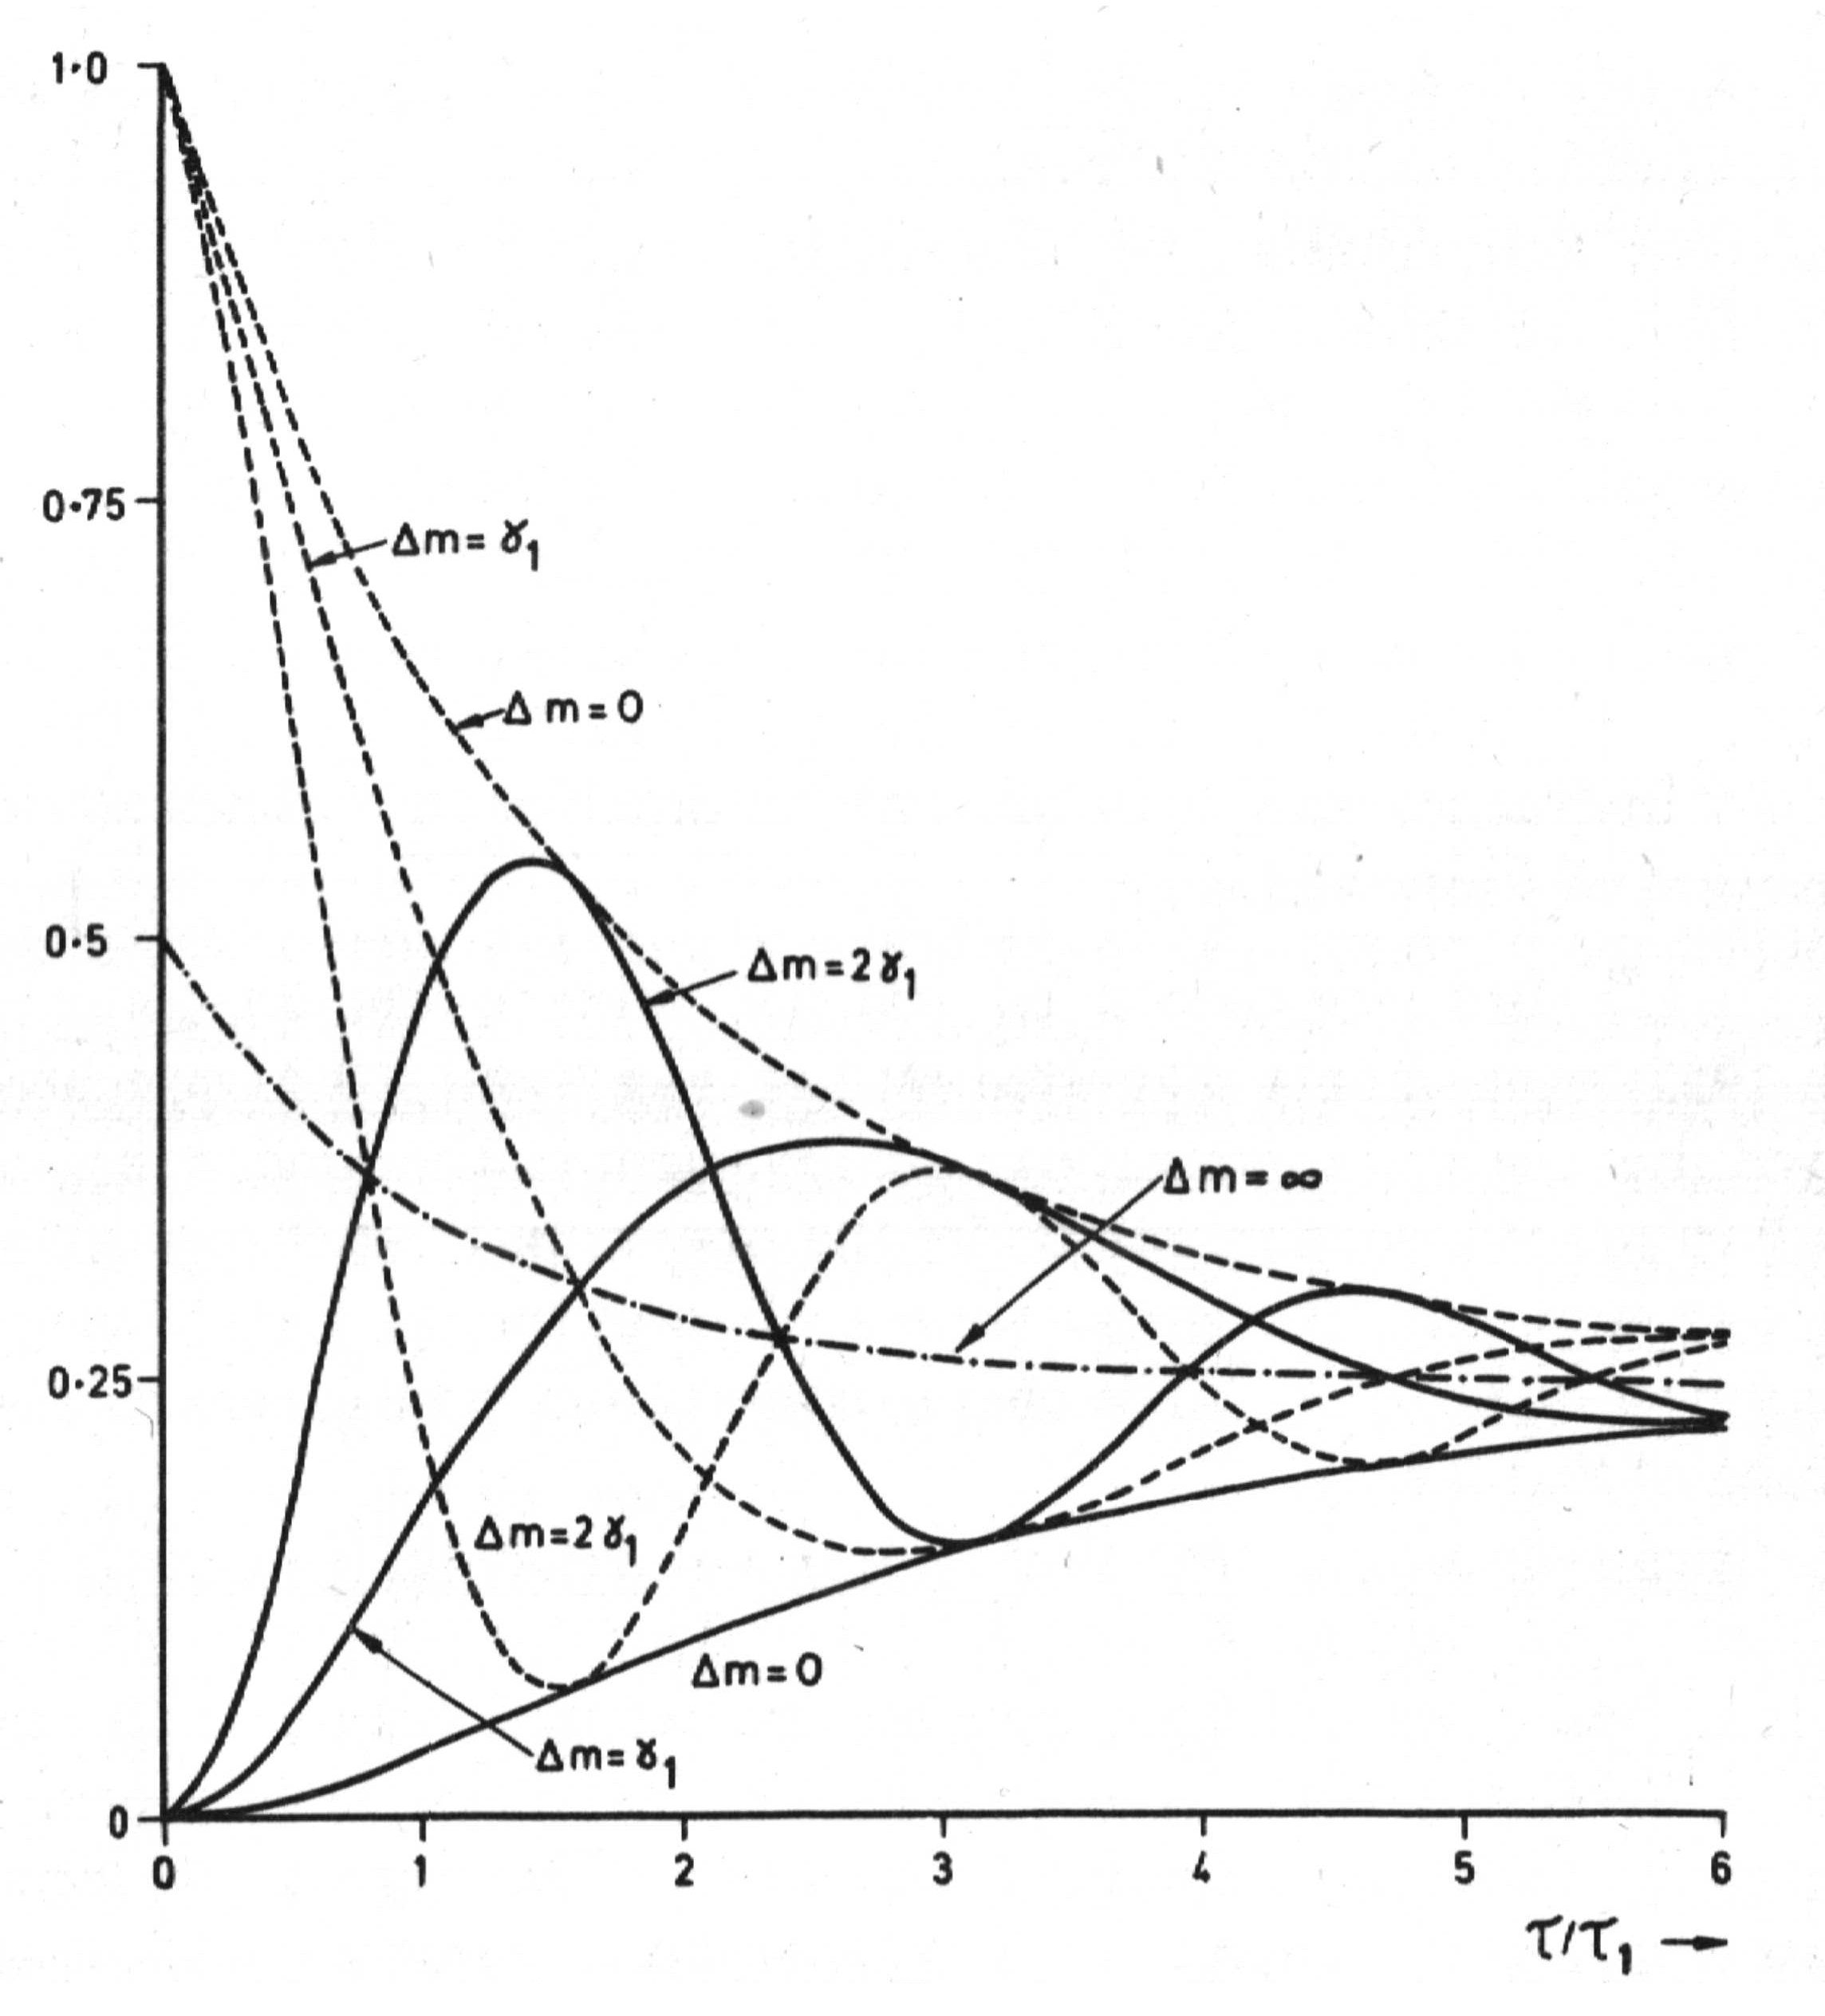
\includegraphics[scale=0.09]{Immagini/oscillazioni}
\caption{Probabilità di trovare un $P^0$ o un $\bar{P}^0$ in un fascio inizalmente costituito dal solo $P^0$ in funzione del tempo, per vari valori di $\Delta m$, la differenza
di massa tra i due autostati di propagazione $P_L$ e $P_S$ \cite{Kabir}.}
\end{center}
\end{figure}

\section{Violazione di CP}
\noindent
In questo paragrafo si studierà la violazione di CP del sistema dei mesoni neutri. Si premette la dimostrazione di due risultati
che saranno fondamentali per la discussione successiva.
\begin{teorema}
 Se il sistema dei mesoni neutri è invariante per CPT allora, indipendentemente dall'invarianza per T, valgono le relazioni:
\begin{equation}\label{teo1a}
 |P_S\rangle = \binom{1+\epsilon}{1-\epsilon} \frac{1}{\sqrt{2(1+{|\epsilon|}^2)}}
\end{equation}
\begin{equation}\label{teo1b}
 |P_L\rangle = \binom{1+\epsilon}{\epsilon-1} \frac{1}{\sqrt{2(1+{|\epsilon|}^2)}}
\end{equation}
dove $\epsilon \in \mathbb{C}$.
\end{teorema}
\begin{proof}
Consideriamo la matrice $H_{eff}$ \eqref{Heff}. Essendo questa una matrice $2 \times 2$ ad elementi complessi, è sempre possibile esprimerla come:
\begin{equation} \label{unimport}
 H_{eff} = D\mathbb{I} + \sum_{i=1}^{3}E_i\sigma_i
\end{equation}
dove $D, E_i \in \mathbb{C}$ sono costanti, mentre le $\sigma_i$ sono le matrici di Pauli \eqref{sigma1}, \eqref{sigma2}, \eqref{sigma3}.
Come è stato già evidenziato, a causa del Teorema CPT gli elementi sulla diagonale principale dell'Hamiltoniana efficace sono tra loro uguali.
Questo porta necessariamente a $E_3 = 0$.
Posto $E_1 = E \cos (\alpha)$ e $E_2 = E\sin(\alpha)$, con $E \in \mathbb{C}$ e $\alpha \in [0,2\pi]$, l'equazione \eqref{unimport} diventa:
\begin{equation}
 H_{eff} = D\mathbb{I} + E \Bigg(\begin{matrix} 0 & e^{-i\alpha} \\ e^{i\alpha} & 0 \end{matrix}\Bigg)
\end{equation}
Si verifica che gli autovettori sono:
\begin{equation}\label{eti}
 \binom{1}{e^{i\alpha}}\ \ \ \ \ \ \ \ \ \ \ \ \ \ \ \binom{1}{-e^{i\alpha}}
\end{equation}
Introducendo la notazione:
\begin{equation}
 e^{i\alpha} = \frac{1 - \epsilon}{1+\epsilon}
\end{equation}
gli autovettori \eqref{eti} diventano:
\begin{equation}
 \binom{1+\epsilon}{1-\epsilon}\ \ \ \ \ \ \ \ \ \ \ \ \ \ \ \binom{1+\epsilon}{\epsilon-1}
\end{equation}
che, divisi per gli opportuni coefficienti di normalizzazione, coincidono con le espressioni \eqref{teo1a} e \eqref{teo1b}.
\end{proof}
%
%
\begin{teorema}
 Se il sistema dei mesoni neutri è invariante per T allora, indipendentemente dall'invarianza per CPT, valgono le relazioni:
\begin{equation}
 |P_S\rangle = \binom{1+\delta}{1-\delta} \frac{1}{\sqrt{2(1+{|\delta|}^2}}
\end{equation}
\begin{equation}
 |P_L\rangle = \binom{1-\delta}{-(1+\delta)} \frac{1}{\sqrt{2(1+{|\delta|}^2}}
\end{equation}
dove $\delta\in \mathbb{C}$.
\end{teorema}
%
\begin{proof}
Per ipotesi la dinamica del sistema è invertibile rispetto all'inversione temporale. Ciò equivale a chiedere:
\begin{equation}
 \langle P_L|M-\frac{i}{2}\Gamma|P_S\rangle = \langle P_S|\mathscr{T}^{-1}(M-\frac{i}{2}\Gamma)\mathscr{T}|P_L\rangle = \langle P_S|M-\frac{i}{2}\Gamma|P_L\rangle
\end{equation}
Ricordando che $|P_L\rangle$ e $|P_S\rangle$ sono autostati dell'Hamiltoniana efficace di autovalori $\mu_L$ e $\mu_S$ si ottiene:
\begin{equation}
 \mu_S \langle P_L|P_S\rangle = \mu_L \langle P_S|P_L\rangle
\end{equation}
Poiché si è dimostrato che $\mu_L \neq \mu_S$, mentre $\langle P_L|P_S\rangle = \langle P_S|P_L\rangle$ si ottiene:
\begin{equation}
 \langle P_L|P_S\rangle = 0
\end{equation}
Due vettori complessi mutualmente ortogonali possono essere parametrizzati nel modo seguente:
\begin{equation}\label{q}
 |P_S\rangle \varpropto \binom{1 + \delta}{1 - \delta}
\end{equation}
\begin{equation}\label{w}
 |P_L\rangle \varpropto \binom{1 - \delta}{-(1 + \delta)}
\end{equation}
con $\delta \in \mathbb{C}$. Le relazioni \eqref{q} e \eqref{w}, divise per gli opportuni fattori di normalizzazione, forniscono la prova dell'asserto. 
\end{proof}
%
% eta
%
A questo punto si definisce il parametro $\eta$ nel modo seguente:
\begin{equation}
 \eta = \langle P_S|P_L\rangle
\end{equation}
in base ai risultati dei due teoremi appena dimostrati si deduce che 
\begin{displaymath}
\left\{
\begin{array}{l}
CPT \Longrightarrow \eta  \ reale\\
T \Longrightarrow \eta \    immaginario
\end{array}
\right.
\end{displaymath}
Infatti se il sistema \`e invariante per CPT dal Teorema 2.1si ha:
\begin{equation} 
\langle P_S|P_L\rangle = \frac{\epsilon + \epsilon^*}{1 + (|\epsilon|)^2}
\end{equation}
mentre se \`e invariante dal Teorema 2.2 per T:
\begin{equation}
 \langle P_S|P_L\rangle = \frac{\delta^* - \delta}{1 + (|\delta|)^2}
\end{equation}
Per cui $\eta$ si rivela un ottimo parametro per valutare la violazione di CP (che, per il teorema CPT, avviene se viene violata T).
Se entrambe le simmetrie CPT e CP fossero esatte, allora si dovrebbe avere $\eta = 0$ e i due autostati $|P_S\rangle$ e $|P_L\rangle$
si ridurrebbero agli autostati dell'operatore $\mathscr{C}\mathscr{P}\ |P_1\rangle$ e $|P_2\rangle$ definiti, nel caso dei kaoni, dalle espressioni \eqref{K1} e \eqref{K2}.
Il parametro $\eta$ può essere calcolato a partire dagli elementi delle matrici di massa e di decadimento. Dato il problema agli autovalori per l'hamiltoniana efficace:
\begin{equation}
(M - i \frac{\Gamma}{2})|P_j\rangle = (m_j - \frac{i}{2} \gamma_j) |P_j\rangle
\end{equation}
Dove $j$ è un indice che può significare $L$ o $S$.
Moltiplicando per l'unità immaginaria i due lati di questa espressione ed eseguendo il prodotto scalare per il bra $\langle P_k|$ (con $k = L, S$) si ottengono le relazioni:
\begin{equation}
 \langle P_S | \frac{\Gamma}{2} + iM | P_L \rangle = (\frac{1}{2} \gamma_L + i m_L) \langle P_S |P_L\rangle 
\end{equation}
\begin{equation} \label{questa}
 \langle P_L | \frac{\Gamma}{2} + iM | P_S \rangle = (\frac{1}{2} \gamma_S + i m_S) \langle P_L |P_S\rangle 
\end{equation}
L'espressione hermitiana coniugata dell'equazione precedente è:
\begin{equation}
 \langle P_L | \frac{\Gamma}{2} - iM | P_S \rangle = (\frac{1}{2} \gamma_S - i m_S) \langle P_L |P_S\rangle 
\end{equation}
che, sommata alla \eqref{questa}, diventa:
\begin{equation}
 2\langle P_S |\Gamma | P_L \rangle = [\frac{1}{2} (\gamma_L + \gamma_S) + i(m_L - m_s)] \eta
\end{equation}
 dove si è usata la definizione $\eta = \langle P_S|P_L \rangle$.
È possibile dimostrare \cite{Lee} la seguente identità:
\begin{equation}
 \langle P_S |\Gamma |P_L \rangle = \frac{1}{2} \sum_c \sqrt{\gamma_S(c)\gamma_L(c)} e^{i\theta_c}
\end{equation}
dove $c$ è un indice che identifica gli stati di decadimento finali, mentre $\phi$ è una generica fase.
Quindi si ottiene la seguente espressione di $\eta$:
\begin{equation}
 \eta = \frac{\sum_c \sqrt{\gamma_S(c)\gamma_L(c)} e^{i\theta_c}}{\frac{1}{2} (\gamma_L + \gamma_S) + i (m_L - m_S)}
\end{equation}
attraverso la quale è possibile quantificare l'entità della violazione di CP in ciascuno dei sistemi $P^0$ - $\bar{P}^0$.